\documentclass{article}
\usepackage{graphicx,subfigure}

\usepackage{arxiv}

\usepackage[utf8]{inputenc} % allow utf-8 input
\usepackage[T1]{fontenc}    % use 8-bit T1 fonts
\usepackage{hyperref}       % hyperlinks
\usepackage{url}            % simple URL typesetting
\usepackage{booktabs}       % professional-quality tables
\usepackage{amsfonts}       % blackboard math symbols
\usepackage{nicefrac}       % compact symbols for 1/2, etc.
\usepackage{microtype}      % microtypography
\usepackage{lipsum}
\usepackage[dvipsnames]{xcolor}
\usepackage{textcomp}
\usepackage{catchfilebetweentags}



\usepackage[shortlabels]{enumitem}
\usepackage{amsmath}
\usepackage{bm}

\usepackage[colorinlistoftodos]{todonotes}

% \usepackage[nomarkers,notablist,nofiglist]{endfloat}
% \usepackage[nomarkers,notablist,nofiglist]{endfloat}
% \usepackage[colorinlistoftodos,disable]{todonotes}


\usepackage[english]{babel}
\usepackage[
backend=biber,
style=nature,
% citestyle=authoryear
]{biblatex}
\addbibresource{references.bib} %Imports bibliography file



\title{evidence of stationary and non-stationary clustered time-warped spike timing in cortical networks}


\author{
  James B. Isbister\\
  University of Oxford, United Kingdom
%   \thanks{Oxford Centre for Theoretical Neuroscience and Artificial Intelligence, University of Oxford, UK.}    
% \thanks{Blue Brain Project, EPFL, Switzerland.}\\
%   University of Oxford, UK.\\
%   EPFL, Switzerland.\\
%   \texttt{james.isbister@psy.ox.ac.uk}\\
%   \textit{isbisterjb@gmail.com}\\
  \And
              \\
              \\
  \And
  Vicente Reyes-Puerta\\
  Johannes Gutenberg University, Germany
  
%   \And
%   Irina Higgins\\
%   DeepMind

  \And
  Jyh-Jang Sun\\
  NERF, Belgium

  \And
  Heiko J. Luhmann\\
  Johannes Gutenberg University, Germany


}


\begin{document}
\maketitle
 
\begin{abstract}
% http://blogs.nature.com/naturejobs/2014/11/03/how-to-get-published-in-high-impact-journals-big-research-and-better-writing/
% \color{blue}`Do not undersell your research. “If you find something big, tell us!'\color{Black} 

REL: Efficient population coding of naturalistic whisker motion in the ventro-posterior medial thalamus based on precise spike timing

Sensory stimulation induced patterns of action potentials recorded in adult rat cortex in vivo allow investigation of neural coding principles. 

Patterns of action potentials induced by sensory stimulation in vivo allow investigation of neural coding principles. Trial-to-trial variability engenders debate over temporal and rate codes. Characterising distributions of stimulus responses enables discovery of response properties, which reliably encode the stimulus and may affect other processes. Non-stationarity (i.e. trial dependence) and noise correlations complicate such characterisation. A novel algorithm found correlated clusters above chance in first spike stimulus-response distributions for pairs of barrel cortex units. First spike times covaried at angles different from $45^{\circ}$ for a proportion of stationary and non-stationary (after removal of trial-dependence) clusters, suggestive of an underlying factor warping the distribution of decodable relative spike time differences from trial-to-trial. Factor analysis allowed estimation of factor-dependent and trial-independent stimulus response distributions, with a high estimated potential for discriminable stimulus encoding. The results suggest that consideration of clustering, factor-dependence and non-stationarity, together, are necessary to explain a large proportion of neural variability.


\end{abstract}


\keywords{Neural coding, precise spike timing, time-warp, feature-binding, barrel cortex, noise correlations, neural adaptation, in vivo recording}


\section{Introduction}
The neural coding problem asks how information is encoded through patterns of action potentials in the nervous system \cite{gerstner1997neural, johnson2000neural, stein2005neuronal, gerstner2014neuronal}, with a dichotomy between temporal \cite{uzzell2004precision, johansson2004first, gollisch2008rapid, storchi2012comparison, reinagel2002precise, reyes2014laminar} and rate codes \cite{hong2016explicit, chang2017code, kar2019evidence, stringer2019high}. 
% Temporal codes provide the possibility of a fast and efficient code. 
Whilst precise temporal patterns have been observed \cite{uzzell2004precision, johansson2004first, gollisch2008rapid, storchi2012comparison, reinagel2002precise, reyes2014laminar}, a large proportion of neural variability remains unexplained. Such variability leads to the common assumption of average firing rate codes, under the premise that variability cancels out across a population \cite{abbott1999effect, moreno2014information, stringer2019high}. Continuous firing rates (averaged over time, trial or population \cite{gerstner1997neural}) have capacity beyond the single trial discrete spike count from which they are abstracted, leaving a full understanding of neural coding and variability undetermined. It is important to better characterise neural codes in order to understand a rich variety of dynamic, structural, homeostatic and cognitive processes, as well as properties of action potential patterns directly involved in behaviour.
% Characterising responses may also uncover response properties involved in behaviour. 

Responses following sensory stimulation can be analysed to explore principles of neural coding. Due to response variability, characterising the neural representation of a single stimulus is a matter of characterising the \textit{distribution} of possible neural responses for the stimulus. A multi-neuron response can be expressed as a point in multi-dimensional space, where each dimension represents a spike train metric. Responses from multiple presentations of a stimulus form a sample stimulus-response distribution in this space (Fig. 1a). 
% which approximates an underlying stimulus-response distribution. 

\begin{figure}[t!]
\centering
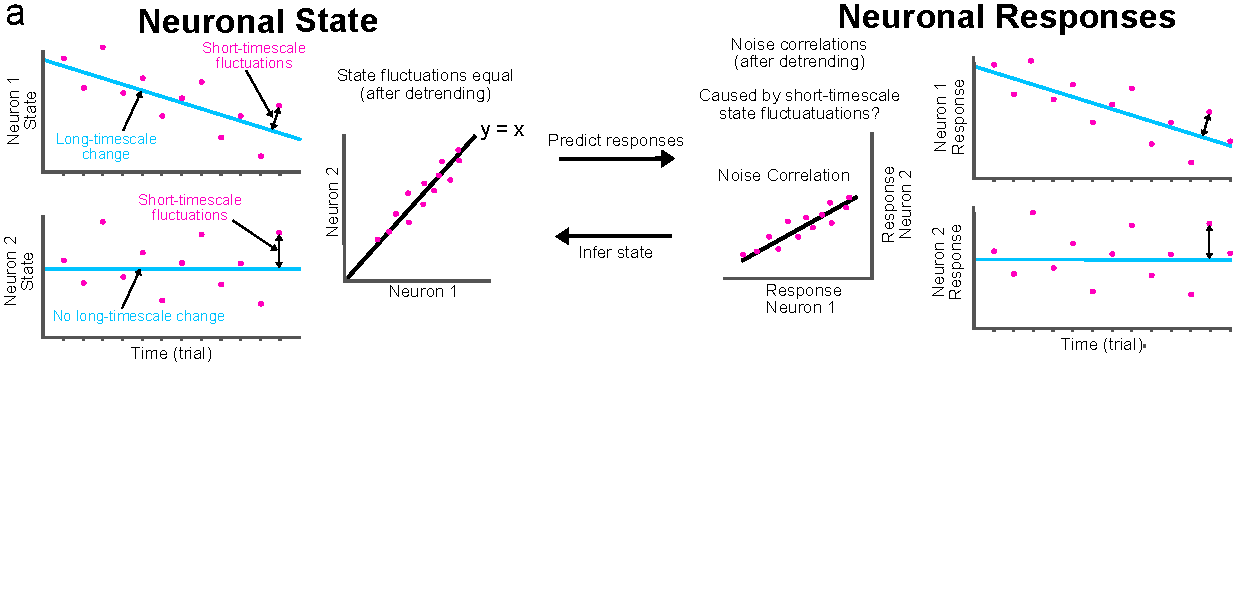
\includegraphics[width=\textwidth]{Figure1.pdf}
\caption{Explanatory Figures. 
(a) Left: For two neurons (x and y-axis), illustration of sample (dots) and boundary of underlying (circle) first spike stimulus-response distributions for two hypothetical stimuli (red and gold). Right: Illustration of corresponding relative first spike differences. 
(b) Illustration of trial dependence of a sampled response distribution (dots). Circle illustrates the boundary of a possible trial-dependent response distribution on a single trial. 
(c) Illustration of boundary of state-dependent first spike response distribution for a single state value. The green line shows the mean points that would be predicted for a continuous set of state values.
(d) Illustration of superposition of two single spike pattern feature representations.
(e) Illustration of `stationary clustered time-warped precise spike timing'. Left: Responses form several clear clusters. The main green cluster is correlated with non-unitary gradient (i.e. different from $45^{\circ}$). Under the assumption of stationarity, the green line and circle are the same as in (c). The orange ellipses illustrate the boundary of an underlying response distribution under the assumption of independence and normality for the sample (solid) and another stimulus (dashed). Centre: Illustration of spike time differences for values of the state. The green circle illustrates the boundary of a state-dependent distribution of spike time differences. Right: Conceptual illustration of time warp relative differences.}
\label{fig:fig1}
\end{figure}

If two stimuli have a behaviourally relevant difference, downstream neurons must be able to respond differently to samples from the response distribution of either stimulus. This is possible if the response distributions are highly non-overlapping in dimensions that downstream neurons are sensitive to, such as relative spike time differences (\cite{gasparini2006state, branco2010dendritic, branco2011synaptic}; Fig. 1a). Characterising the distribution from which a stimulus response is `drawn' from on a single trial is complicated by state dependence, neural adaptation and heterogeneity of sample response distribution structure.

Firstly, correlative structure between the responses of spatially distanced neurons (see \cite{reid2012functional, feldmeyer2013barrel}) in a single stimulus response distribution, opens the possibility of a \textit{continuous} underlying state, which covaries neural responses from trial-to-trial. Response samples on a single trial, when the continuous state has a certain value, would then come from a state-conditioned stimulus-response distribution. This would be a smaller region of stimulus-response space than the region from which all samples come (Fig. 1c). Therefore, if downstream neurons could respond in a state-dependent manner (contrary to common neural coding assumptions \cite{moreno2014information, stringer2019high}), state-dependent encoding would increase the capacity for discriminable stimulus encoding.

Characterisation of response distribution structure is also complicated by neural adaptation, which occurs across species and modalities \cite{dragoi2002dynamics, ulanovsky2003processing, sharpee2006adaptive}, and in barrel cortex to repetitive whisker stimulation for spike count \cite{ahissar2000transformation, ahissar2001temporal, kheradpezhouh2017response, khatri2009stimulus, martin2014tactile, barros2019response} and spike latency \cite{ahissar2000transformation, ahissar2001temporal, kheradpezhouh2017response}. That is, the response distributions are \textit{non-stationary} and change as a function of trial index for some neurons. Adaptation could therefore lead to correlative structure in single stimulus response distributions. Adaptation must therefore be controlled for when searching for correlative structure indicative of a possible underlying state.

The topographic representation of each single whisker on the snout of a rodent in the somatosensory cortex, the so-called barrel cortex, represents an excellent model to study neuronal processing of defined sensory stimulation \cite{feldmeyer2013barrel}. The shortness of whisker deflections reduces ambiguity in what temporal aspect of a stimulus neural activity represents, offering controlled study of the neural representation of atomic entities. The majority of barrel cortex neurons respond 0 or 1 times to single whisker deflections \cite{reyes2014laminar}, implicating single spike patterns as a candidate for atomic representation of information. Representation by single spike patterns is supported in other sensory modalities, such as vision, where a recent optogenetics study showed that early visual cortex patterns of single spikes are sufficient to enable visual discrimination \cite{resulaj2018first}.

First spike times with millisecond order precision have been observed relative to stimulus onset in sensory organs \cite{johansson2004first, uzzell2004precision, gollisch2008rapid}, thalamic areas \cite{reinagel2002precise, storchi2012comparison} and early sensory cortices \cite{reyes2014laminar}, as well as relative to oscillations \cite{havenith2011synchrony}. Relative differences \cite{izhikevich2006polychronization} observed experimentally \cite{johansson2004first, gollisch2008rapid, reyes2014laminar} have been shown to encode information when trial averaged \cite{gollisch2008rapid} and do not require reference to an onset signal.
Response distributions may form multiple clusters, implying stochasticity in the cluster from which representations come on a single trial (Fig. 1d; \cite{reyes2014laminar}).
% as neurons are sensitive to the spatial and temporal pattern of synaptic activations \cite{gasparini2006state, branco2010dendritic, branco2011synaptic}.

Using a large data set of spike sorted recordings in anesthetized rat barrel cortex, first spike response distributions were first observed for single stimuli and pairs of units. That is, for repeated trials of a single stimulus, the first spike times of two units were plotted against each other for trials on which they both spiked. The reader is strongly recommended to view these plots in the top left of Supplementary Vid. 1. Simple observation of these plots (ignoring lines, colours and ellipses at this stage) shows that clusters of first spike pair responses appear correlated, suggesting that first spike pairs are correlated for pairs of neurons on a subset of trials of a stimulus. 

% That is, each axis corresponds to the first spike time of a different recorded unit. The scatter points therefore represent the first spike times of both units for the trials (of a single stimulus) on which both units spiked. 

Moreover, the correlation angle of some of the correlated clusters appears to be different from $45^{\circ}$ (i.e. has a gradient different from 1).
A simple shift in the precise timing of stimulus onset or the onset of cortical activity, would produce correlations with a unitary gradient (i.e. a $45^{\circ}$ angle). The observed correlations with `non-unitary gradient' may suggest that correlations are due to an internal process, for example, a shared cortical state underlying state-dependent processing. Such correlations with `non-unitary gradient' must be considered after checking and controlling for neural adaptive trends.

A novel algorithm extracted the observed clusters and found that they were correlated above chance levels. To control for adaptive trends, the cluster spike times of each neuron in the pair were tested for stationarity. The cluster spike times of both units were stationary for X\% of correlated clusters. X\% of these stationary correlated clusters had non-unitary (different from $45^{\circ}$) correlation angles, suggestive of an internal underlying state co-varying first spike times and thus \textit{warping} the distribution of (decodable) relative spike time differences from trial-to-trial (Fig. 1d).

For the remaining clusters, with at least one unit with non-stationary cluster spike times, time series analysis was applied to remove the neural adaptive trends of the non-stationary unit/units. X\% of the detrended clusters were correlated with non-unitary gradient, suggestive of an underlying state.

Application of state analysis to the stationary and detrended clusters provided an estimate of possible state-dependent response distributions. This gave a prediction of the resolution of possible state-dependent encoding, which would surpass previously proposed coding forms and controls for neural adaptive trends. It also provides a precise understanding of stimulus responses and correlative variability, which could be interpreted classically (i.e. independently of state [Vicente Refs]).

The precise characterisation of correlative structure in this paper is a necessary component step towards either rejecting state-dependent coding, or confirming its precise nature. It is important for neurophysiology to determine whether correlative structure between spatially distanced neurons is caused by continuous state, which also modulates downstream decoding neurons. Testing the state-dependent decoding performance of the response properties uncovered in this paper would require explicit knowledge (or an estimate) of the underlying trial-to-trial state so is left for future studies.
Subthreshold membrane potentials are a candidate for such state, as they affect action potential initiation \cite{petersen2003interaction} and are correlated across areas \cite{poulet2008internal}.

The characterised response distribution structure is referred to as `stationary and non-stationary clustered time-warped spike timing'. This differs from previous `time-warp' studies, which aim to align spike trains over trials and do not consider discriminable encoding, clustering, non-stationarity and different warping functions for different neurons \cite{williams2020discovering}. One previous study has modelled time-warp-invariant integration \cite{gutig2009time}, although neurons need not respond identically to warps of the same pattern. Rather, neurons should process relative spike patterns in a state-dependent manner.

The results suggest that consideration of clustering, state-dependence and non-stationarity, together, are necessary to explain a large proportion of neural variability, and could explain the failure to find a fast and efficient ubiquitous spike code that utilises the high sensitivity of neural architecture and functional dynamics. In this study, such consideration gave a novel prediction of the resolution of neural stimulus representation. 

% To our knowledge this is the first report demonstrating that 

% Algorithms for detecting correlated clusters and estimating correlation angles were developed for this study and verified on surrogate control datasets.


% It follows that the region of response-distribution space from which a stimulus-response is drawn from at a single point in time is smaller than the region from which samples are drawn from over all trials (Fig. 1b). 

% The paper presents a novel technique for uncovering correlated first spike times for pairs of neurons in noisy response distributions. 


% As \textit{spike counts} show high trial-to-trial variability, single units cannot reliably encode many different stimuli, leading to the use of firing rate codes (as discussed above and in the the Discussion).

% Assumptions about stimulus-response distribution structure constrain the potential encoding power of timing-based single spike patterns.
% Independent and normally distributed first spike-times would confer a low discriminability potential (as will be seen), dependent on single neuron variability (Fig. 1e). 
% % Over typical 10-40ms ranges of mean first spike times for short stimuli \cite{reyes2014laminar, resulaj2018first}, 
% % Observed first spike time standard deviations \cite{reyes2014laminar} would imply that very few unique stimuli/features could be encoded with high discriminability by a neuron pair. 
% Spike time differences between two neurons with independent and normal first spike times would have a standard deviation of \(\sigma_{diff} = \sqrt{\sigma_{0}^2 + \sigma_{1}^2}\), where \(\sigma_{i}\) is the standard deviation of neuron $i$ ($i=0,1$).
% Spike times could covary with unitary gradient under the assumption that relative spike times have a factor-independent mean. 
% Precise relative differences have been reported in the eye \cite{gollisch2008rapid} and barrel cortex \cite{reyes2014laminar}. 

% The paper uncovers interesting correlative properties, which offer a novel description of neural representations and are suggestive (but not confirmatory) of an internal continuous state varying responses from trial-to-trial. 

% Using a large data set of spike sorted recordings in anesthetized rat barrel cortex, the paper aims to address the following questions:

% \textit{1.} To repeated repeated trials of single stimuli (i.e. single whisker deflections at a particular velocity) do the first spike times of pairs of units form clear clusters? 


% Firstly, for repeated trials of single stimuli (i.e. single whisker deflections at a particular velocity), are the first spike times of pairs of units correlated? This analysis should take into account outliers and the possibility that responses come .

% In first-spike stimulus-response distributions for pairs of units, correlated clusters were found above chance-levels. Clustering was necessary for the detection of a large proportion of correlations.

% \textit{2.} For sets of correlated spike pairs, are the angles of correlation significantly different from $45^{\circ}$ (i.e. is the gradient of correlation different from 1)? This question is of interest for two reasons. Firstly such . This leads to the 

% \textit{3.} Does this offer a potential improvement in encoding capacity

% \textit{4.} For pairs of units in which
    
% we addressed the following questions / hypotheses. (1) …. (2) …. (3)…


% Although the study analyses responses to single stimuli in isolation, it also considers the proposed and previously suggested neural codes with respect to feature-binding and continua encoding. 


% , which could be determined by some underlying factor or non-stationarity.


% Characterisation techniques for sparse (low trial count) datasets are often used, which make assumptions about distribution structure, risking fundamental distribution properties and encoding forms being overlooked. 

% Projection of the stimulus-response distribution to a first spike time vs difference space would not decrease the area of the distribution, and thus would not improve discriminability. 


% The standard deviation of spike times and spike time differences would not capture clustering structure, thus underestimating discriminability. If trial-wise cluster was determined by some state, then discriminability given a state, would equal the corresponding cluster's discriminability. 

\section{Results}

\subsection*{Neurophysiology}

The dataset used for this paper is reused from an earlier study, of which analyses and data collection methods have previously been reported \cite{reyes2014laminar}. In summary, extracellular recordings were made in 15 anaesthetised Wistar rats using 16 or 128 electrode silicon probes, inserted perpendicularly into the barrel cortex. Single whisker deflections were made at various frequencies (0.1-10Hz) in blocks, each containing typically 200 trials (sweeps) with an intertrial interval of 5 s (occasionally 10, 15, or 30 s). This was repeated for each of the selected target whiskers (maximum 4). Experimental sessions varied in terms of electrode placement, stimulated whiskers, stimulation frequencies and number of trials per unique stimulus. 7 experimental sessions used single shanks with 16 electrodes, whilst 8 experimental sessions used 8 neighbouring shanks (16 electrodes per shank) covering 2-4 barrel-related columns (median 4). Units were classified as excitatory or inhibitory and assigned to a cortical layers L2/3, L4, L5A and L5B/6 (see Methods \ref{methods:spike_sorting}). Spiking activity is analysed following cortical activation onset, determined as 5.2ms following stimulus onset (Supplementary Fig. 1).



\begin{figure}[t!]
\centering
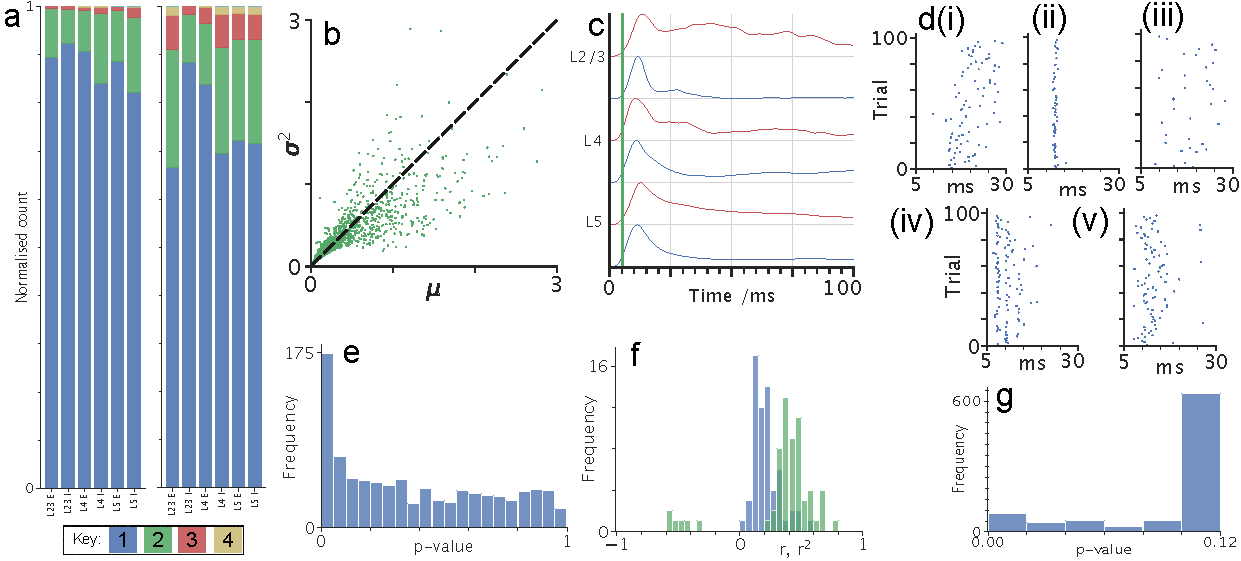
\includegraphics[width=\textwidth]{Figure2.pdf}
\caption{Initial response and first spike time non-stationarity. (a) Spike count histograms (not including 0 spike count) for the 6 neuron groups over 25ms (left) and 100ms (right) following cortical response (responses pooled over all stimuli and trials). (b) Normalised PSTHs following stimulus onset of 6 neuron groups averaged over all stimuli and trials. Cortical onset is marked by the green line. (c) Spike count mean vs variance for all stimuli and unit combinations. (d) First spike rasters following cortical onset for five unit stimulus combinations. (e) P-values of linear regressors fit to predict first spike time from trial index for all stimulus and unit combinations. (f) $R$ (green) and $R^2$ (blue) of linear regressors fit to predict first spike time from trial index for all stimulus and unit combinations. (g) First spike time KPSS p-values for all stimulus and unit combinations. Implementation of p-value estimation rounds all p-values $>0.1$ to 0.1.}
\label{fig:universe}
\end{figure}


\subsection*{Low spike counts}

This section justifies the analysis of first spike patterns as a cortical representation of single whisker deflections. Firstly, this section demonstrates that the majority of neurons respond to single whisker deflections with either 0 or 1 spike (Fig. 2a). Spike count encoding therefore has a low capacity for discriminable stimulus encoding, made worse by high spike count variance (Fig. 2b). The responses of each unit-type and layer group (averaged over stimuli) demonstrate a clear initial response, followed by a tailing-off (Fig. 2c). The paper aims to better characterise this initial (largely single spike) response.


\subsection*{First spike non-stationarity}

This section demonstrates that the responses of some neurons exhibit depressive latency adaption, which should be controlled for when testing for correlative structure caused by a non-adaptive state.

Fig 2d. shows the first spike times of 5 single units in response to repeated presentations of single stimuli. The unit of Fig. 2d(i) demonstrates depressive latency adaptation. The units of Fig. 2d(ii, iii) demonstrate no obvious latency adaptation. The units of Fig. 2d(iv, v) demonstrate more complex response-distribution structure and possible non-linear non-stationarity. For repeated presentations single stimuli, single unit first spike times are linearly correlated with trial number above chance 
(Fisher's method: $\chi^{2} (1786, N = 893) = 3672.69, p<.001$; Fig. 2e).
% (Fisher's method: $\chi^{2} (1786, N = 893) = 3672.69, p = 1.027\textrm{e-132}$; Fig. 2e). 
Of the 63 first spike response distributions that were significantly correlated with trial index (p<.005), $90\%$ (57/63) were positively correlated (Fig. 2f), supporting depressive latency adaptation \cite{ahissar2000transformation, ahissar2001temporal, kheradpezhouh2017response}. The KPSS null hypothesis of stationarity was rejected for p-value < 0.05 for 19\% (168/893) single stimulus single unit first spike response distributions (Fig. 2g). 

Autocorrelations of single-unit single-stimulus first spike times were above chance for lags 1-5 (Supplementary Fig. 2), supportive of general adaptive trends. Only the lag-2 partial autocorrelation was slightly above chance (Supplementary Fig. 2), suggestive of some additional structure in the trial-to-trial sequence of first spike times for some units.
% after accounting for general adaptive trends.


\subsection*{First spike pair response distribution example}

\begin{figure}[t!]
\centering
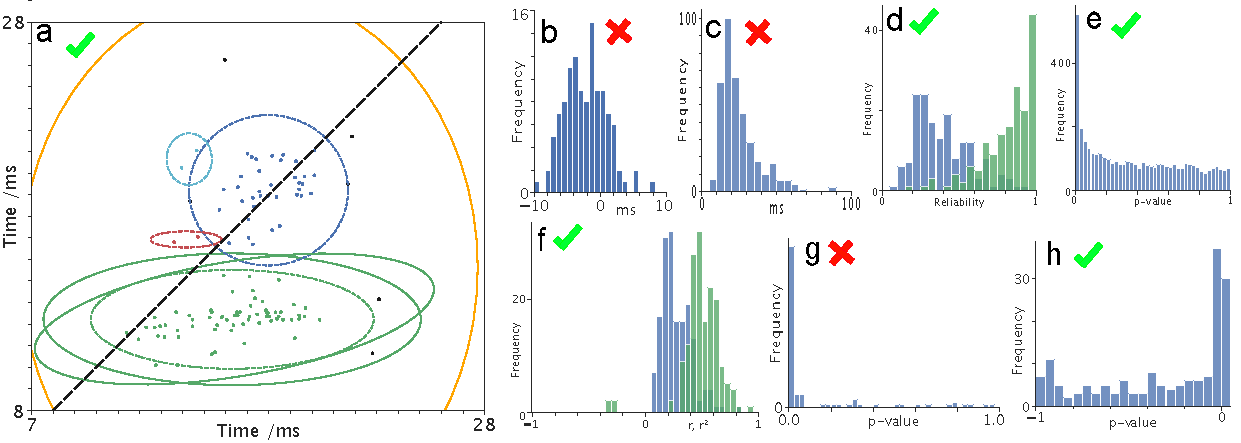
\includegraphics[width=\textwidth]{Figure3.pdf}
\caption{Clustered time-warp example and correlated clusters. (a) Sampled first spike response distribution for two units (L5A Inh, L4 Inh) over a 50ms window following cortical onset (1 outlier out of view). Point colours illustrate DBSCAN cluster (EPS = 1.35). Black points are outliers. Dashed ellipses illustrate $3\sigma$ bounding ellipse calculated for each DBSCAN cluster. Green flat ellipse illustrates $4\sigma$ boundary of green flat cluster. Green angled ellipse illustrates $4\sigma$ boundary of green angled cluster. Orange ellipse illustrates $4\sigma$ ellipse of points under the assumption of independence and normality. (b) Distribution of spike pair differences for response distribution of (a). (c) Histogram of flat cluster end points (mean + $4\sigma$) for all criteria fulfilling angled clusters. (d) The blue histogram represents the ratio of cluster spike pairs to the number of trials of the stimulus, for each angled cluster. The green histogram represents the ratio of cluster spike pairs to the number of trials that both neurons spike to the stimulus, for each angled cluster. (e) Linear regression p-values for all flat clusters. (f) R (green) and $R^2$ (blue) values of all angled clusters. (g) Linear regression p-values of first unit cluster spike times and spike difference. (h) Histogram of flat cluster linear regression p-values minus conjunctive linear regression p-values, for all criteria fulfilling angled clusters.}
\label{fig:fig3}
\end{figure}

Fig. 3a shows the distribution of first spike pairs in response to a 4Hz stimulus for two units (L5A Inh, L4 Inh) over a 50ms window following cortical onset. Only responses on `conjunctive trials' (trials on which both units spiked) are shown. The orange Gaussian is centered at the mean and has widths equal to 4 times the first spike time standard deviations of each unit (on conjunctive trial), illustrating the region from which 99.9\% of first spike pairs would be predicted to fall under the assumption of independence and normality. The assumptions fail to capture the distribution structure of many spike pair distributions (Supplementary Vid. 1) and would allow very few stimuli to be encoded with high-discriminability. The spike time differences have a standard deviation of X (Fig. 3b), which is also poor for discriminable encoding. 

First spike pairs in Fig. 3a appear to form two clusters (blue and green dots). The green cluster appears correlated with non-unitary gradient, suggestive of an underlying factor, which covaries first spike times, such that distributions of differences would be smaller when factor-conditioned, offering a higher power for discriminable encoding. 


\subsection*{Clustering algorithm summary}
A two-stage algorithm was developed to quantify the occurrence and angle of correlated clusters. 
Stage 1 extracted well isolated \textit{`flat clusters'} defined by the $4\sigma$ boundary of flat 2D Gaussian ellipses (flat solid green ellipse in Fig. 3a; see Methods \ref{methods:flat_clusters} for details).  
% The algorithm applied the unsupervised DBSCAN clustering method to first spike response distributions for a range of values of the DBSCAN EPS free parameter. Repeated clusterings for different values of the EPS free parameter were removed from analysis. For DBSCAN clusters that were well isolated and had more than 20 elements, a bounding ellipse was defined from the means and standard deviations of points in the DBSCAN cluster (flat solid green ellipse in Fig. 3a). Points in this bounding ellipse were assigned to the `flat cluster'. 
To assess the occurrence of correlated clusters without sample bias, repeated and similar flat clusters produced by non-identical DBSCAN clusterings were left in the final group of flat clusters (Methods \ref{methods:flat_clusters}). When the algorithm was verified on surrogate control datasets (see Methods \ref{methods:correlation_surrogate_control_datasets}) correlated clusters were found at chance levels (Supplementary Fig. 3). 

Stage 2 of the clustering algorithm aimed to better estimate the shape of the distributions underlying correlated flat clusters (p-value < 0.005), by estimating an `angled cluster' ellipse (angled solid green ellipse in Fig. 3a; see Methods \ref{methods:angled_clusters}). Repeats, similar and non-isolated angled clusters were discarded. 
\ExecuteMetaData[100msAnalysisOutputLatex.tex]{ClusterTimeSpanSummary} \ExecuteMetaData[AnalysisOutputLatex.tex]{AngledClustersUniquePairsSummary}
X\%\todo[color=red!40]{Fill} of angled clusters contained spikes from all conjunctive trials (Fig. 3d).


\subsection*{Correlation analysis}
\ExecuteMetaData[AnalysisOutputLatex.tex]{ClusterCorrelationSummary1}
\ExecuteMetaData[AnalysisOutputLatex.tex]{ClusterCorrelationSummary2}

% The spike time of either neuron would be correlated with the difference \todo[color=green!40]{Figure?}(Fig. X) but due to independence there would be no process underlying this correlation, and thus no means by which downstream neurons could interpret the difference in a state-dependent manner (other than an event signal). Moreover, the discriminability of one neuron's spike time and the difference would be the same as that of the two neuron's spike times \todo[color=green!40]{Same figure}(Fig. X).  


\subsection*{Cluster angle}
\label{results:cluster_angle}

\begin{figure}[t!]
\centering
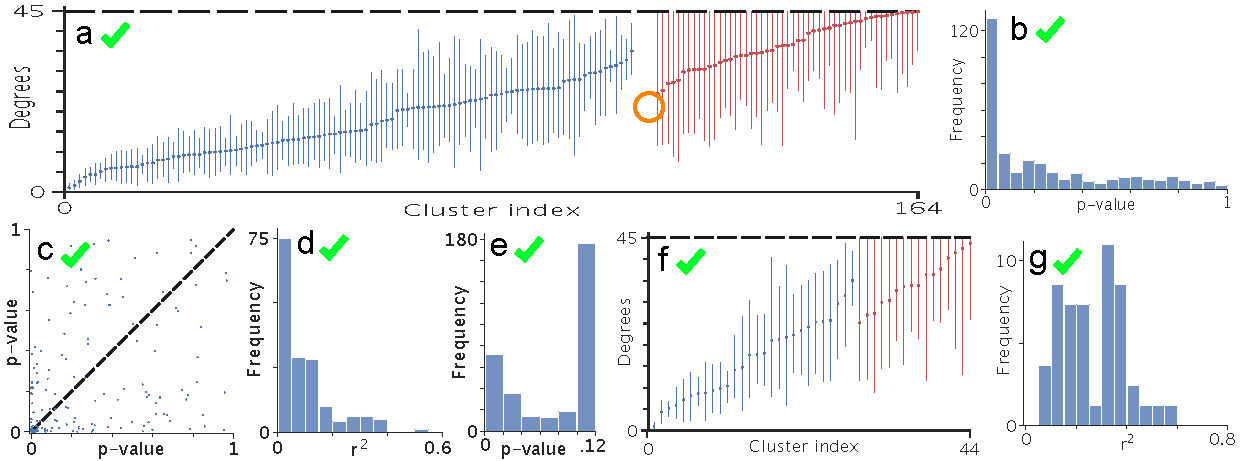
\includegraphics[width=\textwidth]{Figure4.pdf}
\caption{(a) Mean $\theta_{45}$ angles with 95\% confidence intervals for criteria fulfilling positively correlated angled clusters. Angles are coloured blue if they are significantly greater than $0^{\circ}$ (p-value < 0.025) and less than $45^{\circ}$ (p-value < 0.025), and red otherwise. [Gap shown by orange circle to be removed.] (b) Correlation p-values of angled cluster single unit spike times with trial index. (c) Correlation p-values of angled cluster single unit spike times with trial index (unit 0 vs unit 1). (d) $R^2$ values of multi-output regression (trial index vs spike pairs). (e) Cluster single unit KPSS p-values. Implementation of p-value estimation rounds all p-values $>0.1$ to 0.1. (f) Estimated angles of criteria fulfilling angled clusters. (g) Linear regression $R^2$ values for criteria fulfilling angled clusters.}
\label{fig:universe}
\end{figure}

An algorithm was developed to estimate a mean angle and confidence interval for each angled cluster (see Methods \ref{methods:cluster_angle_confidence_interval} for details), to test whether the angles of angled clusters were significantly different from $45^{\circ}$ (possibly indicative of factor or trial-dependent spike time differences). The mean angles, $\theta$, of positively correlated angled clusters (between $0^{\circ}$ and $90^{\circ}$) were of interest. $\theta_{45} = min(\theta, 90-\theta)$ were calculated for analysis, as only the ordering of the units in the pair determined whether $\theta$ was above or below $45^{\circ}$.

\ExecuteMetaData[AnalysisOutputLatex.tex]{OriginalAnglesSummary}
The algorithm was tested on a surrogate control dataset to validate that the detection of such differences from $45^{\circ}$ were not artifacts of the algorithm (see Methods \ref{methods:angle_surrogate_control_dataset}; Supplementary Fig. 6). The following subsections aim to determine when trial number and/or another factor underlie such non-unitary covariation.



\subsection*{Cluster stationarity and normality}

\ExecuteMetaData[AnalysisOutputLatex.tex]{ClusterSingleUnitTrialIndexLRSummary}
Only a small amount of variance was explained by the linear models fit to predict the joint spike pair times from trial number (Fig. 4d), suggesting that neural adaptation may not alone explain the covarying cluster spike times. 
% More complex first spike time relationships with trial index were also observed. 
\ExecuteMetaData[AnalysisOutputLatex.tex]{ClusterSingleUnitKPSSStationaritySummary}

Beside general adaptive trends, some units exhibited observable short trial-by-trial sequences (3-4 trials) of highly correlated first spike times, before losing such correlations. Lagged autocorrelations were significantly above chance for a high number of lags (Supplementary Fig. 4) supportive of general adaptive trends. Only the lag-2 partial autocorrelation was significantly above chance (p-value < 0.005; Supplementary Fig. 4), representative of the additional trial-by-trial structure observed for very few single units.

The cluster spike times of cluster unit pairs exhibit lagged cross-correlations above chance for lags 1-5 (Supplementary Fig. 5), as expected for general adaptive trends. Only the lag-2 partial cross-correlation was above chance (Supplementary Fig. 5). This suggests that the individual adaptive trends of cluster pairs explains the majority of above chance cross-correlations, whilst there may be some finer sequential structure between a few unit pairs. 

% Normality was rejected for X of Y single unit cluster spike times (Shapiro-Wilks p < 0.05; Supplementary Fig. 7) and X out of Y 2-dimensional angled clusters (Henze-Zirkler p < 0.05; Supplementary Fig. 7).




\subsection*{Analysis of stationary clusters}
\ExecuteMetaData[AnalysisOutputLatex.tex]{OriginalTestsPassedSummary}
\ExecuteMetaData[AnalysisOutputLatex.tex]{OriginalTestsPassedAngleSummary}
Fig. 4g shows the amount of variance explained by the stationary angled cluster correlations. Autocorrelations, cross-correlations, partial autocorrelations and partial cross-correlations were at chance levels for the stationary clusters (Supplementary Fig. 7).


\begin{figure}[t!]
\centering
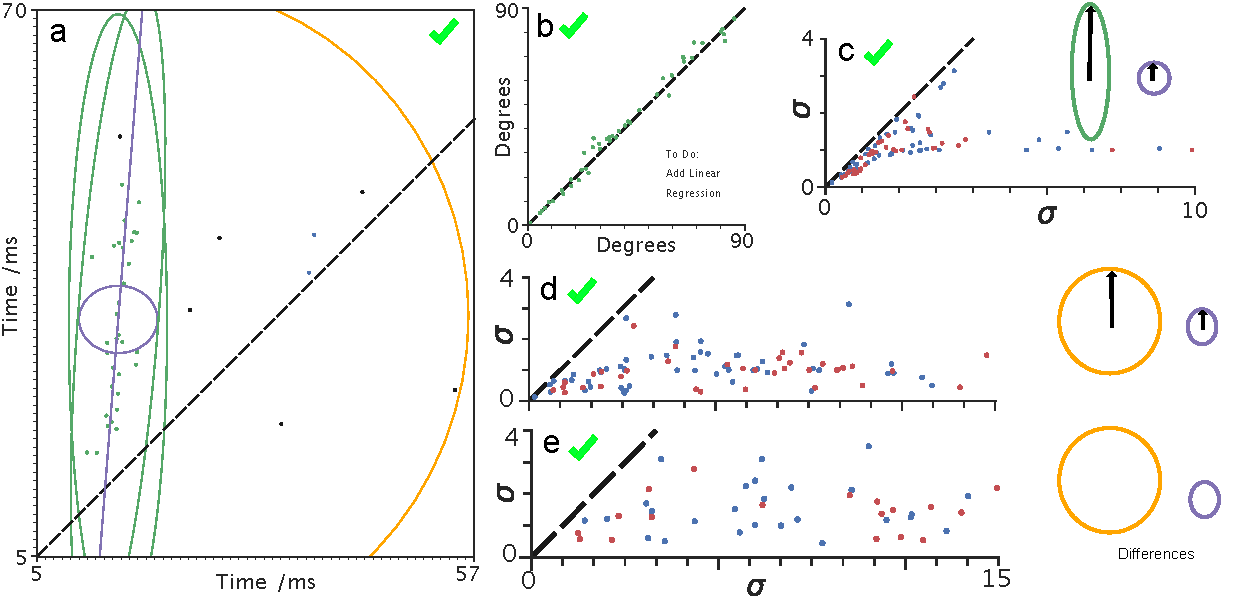
\includegraphics[width=\textwidth]{Figure5.pdf}
\caption{(a) Sampled first spike response distribution for two units (L5B Exc, L5A Exc). Point colours illustrate DBSCAN cluster (EPS = 5.0). Black points are outliers. Green flat ellipse illustrates $4\sigma$ boundary of green flat cluster. Green angled ellipse illustrates $4\sigma$ boundary of green angled cluster. Yellow ellipse illustrates $4\sigma$ ellipse of points under the assumption of independence and normality. Purple circle illustrates the $4\sigma$ boundary of the factor-conditioned response distribution predicted by factor analysis for a single factor value. The purple line shows the mean points predicted for the factor values [-4, 4] (i.e. with variance equal to 0). (b) PCA angles vs factor analysis angles for the criteria fulfilling clusters. (c) The standard deviations of the flat clusters vs standard deviations of the factor-dependent response distributions predicted by factor analysis (for units $i = 0,1$ separately). (d) The standard deviations of the conjunctive trial first spike times vs the standard deviations of the factor-dependent response distributions predicted by factor analysis (for units $i = 0,1$ separately). (e) The standard deviation of differences on conjunctive trials vs the factor-dependent standard deviation of differences predicted by factor analysis.}
\label{fig:universe}
\end{figure}


\ExecuteMetaData[AnalysisOutputLatex.tex]{OriginalTestsPassedFactorAnalysisSummary} The following sections apply time series analysis techniques to remove the neural adaptive trends of the non-stationary units of the remaining clusters. The factor correlation matrix of all criteria fulfilling angled cluster had only one eigenvalue greater than 1, suggesting that a single factor underlied the pairwise cluster covariations. The following single factor model was therefore fit to the elements of each (zero-centered) cluster: $s_i = \lambda_i \eta + \sigma_i$ for $i \in [0, 1]$ 
% and $s_1 = \lambda_1 \eta + \sigma_1$, 
where $\eta$ is some underlying factor, 
% $\lambda_i$ is the gradient at which the factor affects the spike time of unit $i$, 
and $\sigma_i$ is the predicted standard deviation of $s_i$ given $\eta$. Bootstrapping (1000 iterations) was used to calculate means of these values, which were used in subsequent analyses.

The purple line in Fig. 5a shows the values predicted by the model for $\eta = [-4, 4]$ and $\sigma_i = 0$, re-centered around the cluster mean. $\theta_{45}$ angles of the factor lines were estimated using the same method used for PCA component angle estimation (Methods \ref{methods:cluster_angle_confidence_interval}) and were similar to the corresponding PCA $\theta_{45}$ angles (Fig. 5b). The purple ellipse in Fig. 5a has widths equal to $4\sigma_0, 4\sigma_1$ where  $\sigma_0, \sigma_1$ are the standard deviations of the predicted factor ($\eta$) dependent response distribution. This allows visual comparison of the estimated factor-conditioned response distribution to the larger $4\sigma$ areas under the assumptions of normality and independence (orange), normal and independent clusters (green flat cluster) and normal correlated clusters (green angled cluster). 

The areas of the two-dimensional (i.e. two unit) factor dependent response distributions show a striking improvement in potential encoding power (Supplementary Vid. 1; Supplementary Fig. 8). The standard deviations $\sigma_i$ of the factor analysis predicted response distributions for units $i = 0,1$ separately are also strikingly smaller than those assumed by the simpler assumptions (Fig. 5c,d). The factor dependent predicted standard deviations, $\sigma$, are less than 1 for X\% of units and less than 2 for Y\% of units\todo[color=red!40]{Fill}. 
% This gives an estimate of potential encoding power for single units, given by the factor dependent response distributions. 
% It is necessary to consider the results in terms of relative spike timing differences, which can be explicitly processed by downstream neurons.
As the factor analysis model assumes that noise for each unit given $\eta$ is normally distributed and independent between units, the state-dependent difference standard deviation predicted by the model is equal to \(\sigma_{diff} = \sqrt{\sigma_{0}^2 + \sigma_{1}^2}\).
% , where  $\sigma_0, \sigma_1$ are the standard deviations predicted by factor analysis given state $\eta$. 
The estimated $\sigma_{diff}$ values are strikingly lower than the original standard deviation of differences (Fig. 5e). 

% The factor analysis model therefore predicts factor-dependent distributions of differences with a higher potential for discriminable continua encoding than both unclustered spike time differences and clustered but factor-independent spike time differences.



\begin{figure}[t!]
\centering
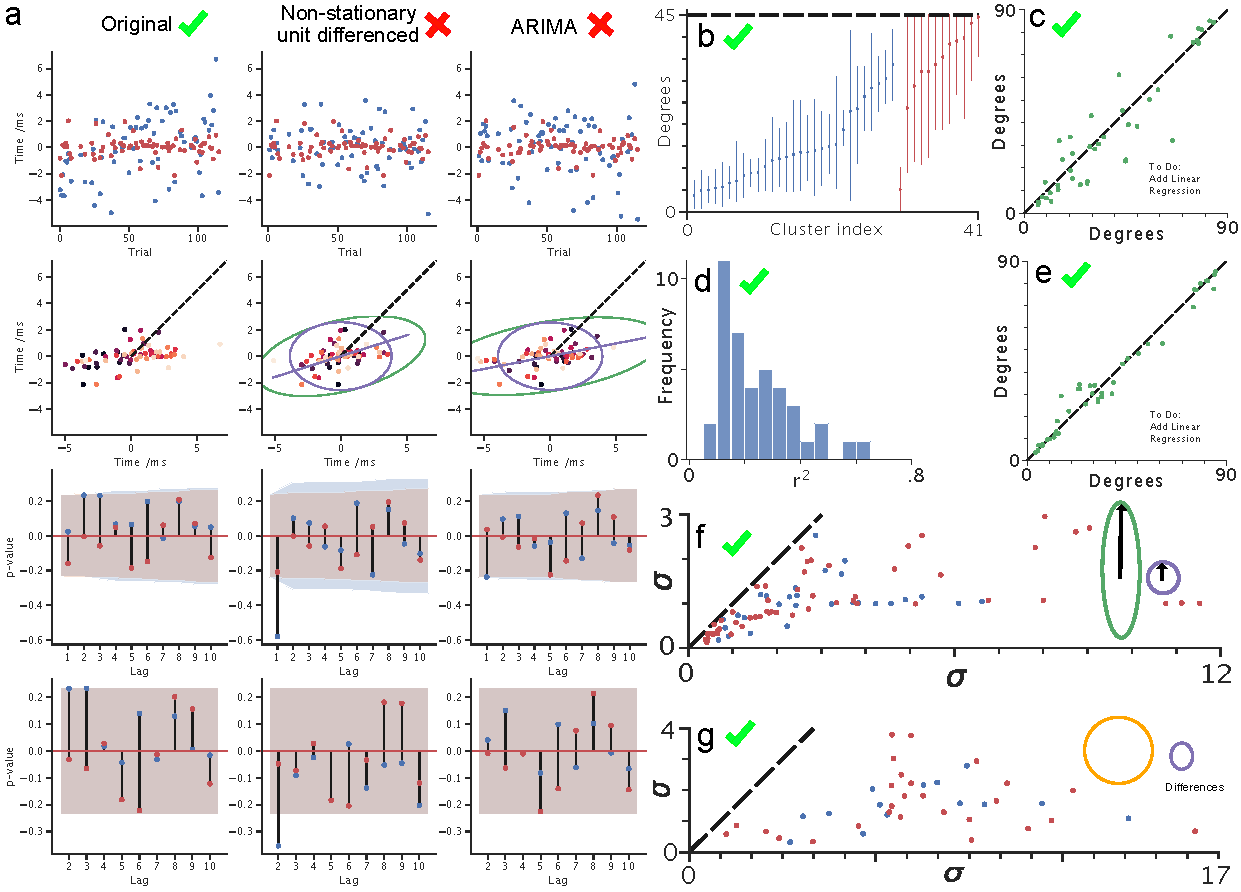
\includegraphics[width=\textwidth]{Figure6.pdf}
\caption{(a) This subfigure analyses the spike times of the green cluster from Fig. 3a for which the spike times of one unit were non-stationary. The columns correspond to (1) the original angled cluster spike times, (2) the cluster after the non-stationary unit cluster spike times were differenced, and (3) the result of applying ARMA modelling to the differenced cluster. Row 1 shows the cluster spike times of both units. Row 2 shows the corresponding cluster, with point colour illustrating trial index (from dark to light). The clusters fulfil the criteria after differencing (autocorrelation criteria relaxed) and ARIMA modelling. As such the $4\sigma$ angled bounding ellipse and factor analysis line and circle are presented. Rows 3 and 4 present the autocorrelation and partial autocorrelation plots respectively with 95\% confidence intervals. (b) Predicted angles and confidence intervals of the criteria fulfilling differenced clusters. (c) Original PCA angles vs differenced PCA angles for the criteria fulfilling differenced clusters. (d) Linear regression $R^2$ values for criteria fulfilling differenced clusters. (e) PCA angles vs factor analysis angles for the criteria fulfilling differenced clusters. (f) The standard deviations of the original flat clusters vs standard deviations of the factor-dependent response distributions predicted by factor analysis for the criteria fulfilling differenced and scaled clusters (for units $i = 0,1$ separately). (g) The standard deviation of the original differences on conjunctive trials vs the factor-dependent standard deviation of differences predicted by factor analysis for the criteria fulfilling differenced and scaled clusters.}
\label{fig:fig6}
\end{figure}



\subsection*{Differencing}

To test whether a shared state could underlie covariation in the remaining non-stationary angled clusters, the non-stationary single unit cluster spike times were differenced and rescaled (a standard time-series analysis technique) to remove neural adaptive trends by subtracting the spike time on trial t by the spike time on trial t-1.
% Clusters which did not fulfil the criteria after differencing were removed from further analysis. 
% Differencing a time series reduces the number of samples by 1 (Methods \ref{methods:angle_and_factor_analysis_criteria}). 
The green angled cluster of Fig. 3a fulfils the criteria after the spike times of its non-stationary unit are differenced (Fig. 6a). Application of the angle estimation technique estimated that the angle was X\todo[color=red!40]{Fill} plus minus Y (Fig. 6a), similar to the original angle and suggestive of an underlying factor after the removal of trial dependence. As expected by differencing, the spike times of the differenced unit show negative lag-1 autocorrelations and negative lag-2 partial autocorrelations (Fig. 6a). 
% Such negative autocorrelations are expected by differencing, and are removed in the next section by fitting ARIMA models.

 
Due to the expected negative autocorrelations introduced by differencing (Supplementary Fig. 9), the criteria for cluster unit autocorrelation p-values < 0.05, was relaxed for the differenced clusters (criterion 6, Methods \ref{methods:angle_and_factor_analysis_criteria}).
\ExecuteMetaData[AnalysisOutputLatex.tex]{SelectivelyDifferencedTestsPassedNewSummary}

\ExecuteMetaData[AnalysisOutputLatex.tex]{SelectivelyDifferencedTestsPassedEigenvalueSummary}
Again, the factor analysis angles show close similarity to the PCA angles (Fig. 6e).
The standard deviations of the factor-dependent response distributions (estimated by factor analysis) again offer a strikingly higher potential for encoding than simpler neural coding assumptions (Fig. 6a; Supplementary Vid 1; Fig. 6f,g; Supplementary Fig. 10).

% Negative lag-1 autocorrelations were found above chance levels but at chance for lags 2-12 (Supplementary Fig. X). Negative partial autocorrelations were found for lags 1-4 above chance levels, and at chance levels for lags 5-12 (Supplementary Fig. X). Such negative autocorrelations are expected by differencing. Positive autocorrelations and partial autocorrelations were found at or below chance for lags 1-12 (Supplementary Fig. X). It was inappropriate to assess cross correlations, which could be spuriously due to autocorrelations.

% \ExecuteMetaData[AnalysisOutputLatex.tex]{SelectivelyDifferencedSummary}

% Differencing removed the correlations of both units' spike times with trial index, as expected by selective differencing criterion 1 (Fig 6b). Selective difference spike times of both units are stationary according to the KPSS test, as expected by selective differencing criterion 2 (Fig 6c). 

% Some Shapiro-Wilks (Fig. 6f). Some Henze-Zeckler normal (Fig. 6g). Most pass spherecity test (Supplementary Fig. X)

% \ExecuteMetaData[AnalysisOutputLatex.tex]{SelectivelyDifferencedCorrelatedSummary}
% \ExecuteMetaData[AnalysisOutputLatex.tex]{SelectivelyDifferencedTestsPassedSummary}




\subsubsection*{ARIMA modelling}


\begin{figure}[t!]
\centering
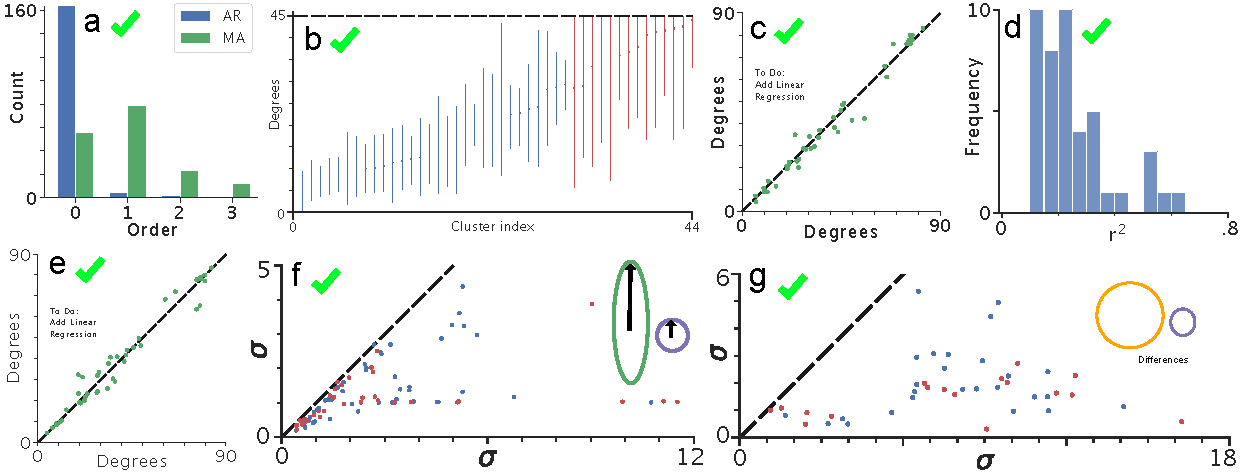
\includegraphics[width=\textwidth]{Figure7.pdf}
\caption{(a) Order of AR and MA models fit to the single unit cluster spike times of differenced clusters. (b) Predicted angles and confidence intervals of the criteria fulfilling ARIMA clusters. (c) Original PCA angles vs ARIMA PCA angles for the criteria fulfilling ARIMA clusters. (d) Linear regression $R^2$ values for criteria fulfilling ARIMA clusters. (e) PCA angles vs factor analysis $\theta_{45}$ angles for the criteria fulfilling ARIMA clusters. (f) The standard deviations of the original flat clusters vs standard deviations of the factor-dependent response distributions predicted by factor analysis for the criteria fulfilling ARIMA clusters (for units $i = 0,1$ separately). (g) The standard deviation of the original differences on conjunctive trials vs the factor-dependent standard deviation of differences predicted by factor analysis for the criteria fulfilling ARIMA clusters.}
\label{fig:universe}
\end{figure}


To remove autocorrelations in cluster unit time series (particularly negative autocorrelations introduced by differencing) and to return the differenced time series to the original scale without division by 2, autoregressive (AR) and/or moving average (MA) models were fit to differenced correlated criteria fulfilling angled clusters, using an automated version of the Box-Jenkins method (Methods \ref{methods:automated_box_jenkins}).
 
\ExecuteMetaData[AnalysisOutputLatex.tex]{SelectivelyDifferencedBoxJenkinsDifferencedSummary}
As expected, the model residuals showed autocorrelations, partial autocorrelations, cross correlations and partial cross correlations at and below chance levels (Supplementary Fig. 11). 
% Overall\todo{What type of clusters? Check.}, a very low amount of variance was explained by the linear models fit to predict spike pair times from trial number (Fig. 7e). 

% The following number of models were fit to single unit cluster time series: MA(1): X/Y, MA(2): X/Y, MA(3): X/Y, AR(1): X/Y, AR(2): X/Y, AR(3): X/Y. 
% Differencing and ARMA removed the correlations of both units' spike times with trial index, as expected by selective differencing criterion 1 (Fig 7c). Selective difference spike times of both units are stationary according to the KPSS test, as expected by selective differencing criterion 2 (Fig 7d). 
% Shapiro (Supplementary Fig. X). Some Henze-Zeckler normal (Fig. 7f). Most pass spherecity test (Supplementary Fig. X)

\ExecuteMetaData[AnalysisOutputLatex.tex]{SelectivelyDifferencedBoxJenkinsCorrelatedSummary}
Fig. 7d shows the amount of variance explained by the pairwise correlation to the criteria fulfilling ARIMA cluster.
Fig. [ToDo] shows the difference between scaled differenced and ARIMA estimated cluster angles, showing that the scaled difference angles gave a good estimation of the angle.

\ExecuteMetaData[AnalysisOutputLatex.tex]{SelectivelyDifferencedBoxJenkinsTestsPassedEigenvalueSummary} 
The angles estimated for the factor analysis components were similar to the angles estimated by PCA (Fig. 7e). The standard deviations of the factor-dependent response distributions (estimated by factor analysis) again offer a strikingly higher potential for encoding than simpler neural coding assumptions (purple ellipses in row 2 column 3 of Supplementary Vid 1; Fig. 7f,g; Supplementary Fig. X).



\subsection*{Stimuli, unit-types and unit-locations}

Fig. 8a shows the spatial distribution of unit pairs which exhibited criteria fulfilling correlated clusters, pooled for stationary clusters and non-stationary clusters made stationary by ARIMA modelling. Correlations are found, which span multiple (up to 4) cortical layers and barrels for both E and I types. The most correlations are found between E-type units in L5A and L5B of the principle column and neighbouring columns. Fig. 8b shows a histogram over stimulus frequencies of criteria fulfilling correlated clusters both for stationary clusters and non-stationary clusters made stationary by ARIMA modelling. 

\begin{figure}[t!]
\centering
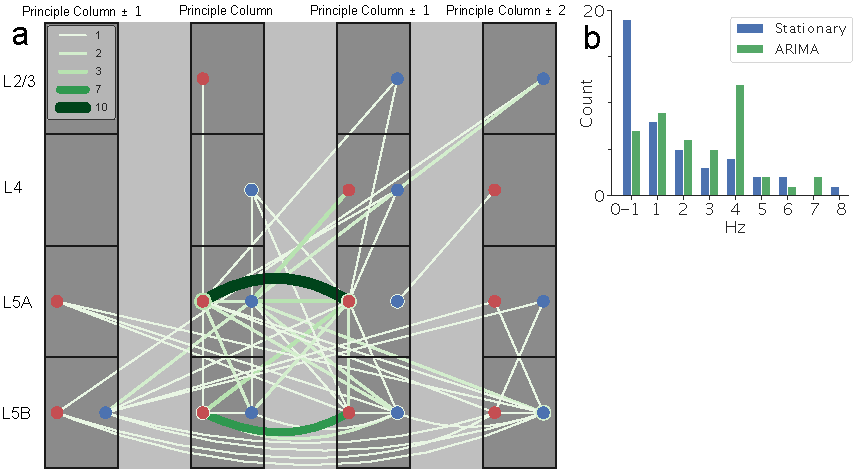
\includegraphics[width=\textwidth]{Figure8.pdf}
\caption{Spatial organisation and eliciting stimuli of criteria fulfilling correlated clusters. (a) Line colour and thickness indicates the number of criteria fulfilling correlated clusters found for pairs of units of different E/I-type and in different layers and barrels. Red and blue correspond to E and I unit types respectively. For example, the thick green line illustrates that there were 10 criteria fulfilling clusters, for which both units were in L5B, 1 unit was in the principle column and 1 was in a neighbouring column. The colour and thickness of rings surrounding the red or blue circles indicate the number of pairs of the same E/I type, layer and barrel. The left most column is shown for pairs in which units in a pair are on opposite sides of the principle column. Counts are pooled for stationary clusters and non-stationary clusters made stationary by ARIMA modelling. (b) Histogram over stimulus frequencies of criteria fulfilling correlated clusters both for stationary clusters and non-stationary clusters made stationary by ARIMA modelling.}
\label{fig:universe}
\end{figure}


% Fig. 8a,b,c show the distribution of pairwise locations for unique correlated secondary clusters for E/E, I/I and E/I unit pairs respectively. It is clear that such pairwise correlations occur across cortical layers and barrels, with X correlations occurring across 4 cortical barrels\todo[color=red!40]{Ellaborate}. This gives primary evidence that a shared state underlying the correlations may at least be shared across Xmm of cortex, making it possible that downstream neurons could process/interpret pairwise differences in a state-dependent manner. The majority of unique secondary correlated clusters occured for low-frequency stimulations (0-4Hz) (Fig. 8d). It is important to note that the heterogeneity in the experiments (i.e. number of trials per stimulus, stimulation frequencies, stimulated whiskers, barrels recorded from, heterogeneity in type and selectivity of units detected) makes it difficult to make full quantitative conclusions as to the spatial distribution of correlated clusters and the stimuli which they are elicited by.





\section{Discussion}

\subsection*{Summary of results}
[TO DO]

\subsection*{Underlying state}
[TO DO]

% For example,  The local field potential (LFP) reflects changes in the subthreshold membrane potential [REF] and is strongly correlatated across cortical layers [REF], suggesting that a subthreshold membrane potential state could be shared across layers.

\subsection*{The feature-binding problem (FBP) and space-time continua}
[TO DO]

It is possible that double spike responses are examples of superpositions of single spike representations, which would increase the encoding capacity further by allowing co-activity of overlapping cell assemblies. 

Action potential instantaneity suggests that relative spike codes could superimpose (Fig. 1d).

some evidence of continuum-like encoding relative to onset \cite{gollisch2008rapid, storchi2012comparison} and oscillations \cite{havenith2011synchrony}.

Trial-averaged firing rate population codes (often calculated over windows $>100ms$) allow decoding of object \cite{hong2016explicit} and face \cite{chang2017code} properties from macaque higher visual areas. 
% Such long integration windows are discordant with behavioural speed \cite{thorpe1996speed} and the fast propagation of activity through cortical layers and areas \cite{perrett1982visual}. 
Object category can be decoded population trial averaged multi-unit activity (MUA) over short 10ms time windows \cite{kar2019evidence}. Decoders do not generalise to later windows \cite{kar2019evidence}, excluding the notion of sustained firing rate representations. Higher encoding capacity is conferred by high spike counts of unsorted MUA \cite{hong2016explicit, kar2019evidence} or for persisting visual stimuli \cite{hong2016explicit, chang2017code, kar2019evidence}. Dimensionality reduction is commonly used to find informative dynamical population firing rate patterns \cite{ahrens2012brain, mante2013context, cunningham2014dimensionality}.
Spike count and firing rates do not superimpose (Fig 1d\todo[color=red!40]{To do}), although competition schemes have been presented for simultaneously active overlapping representations \cite{bao2018representation}. 
% Rate and timing codes may be aligned to internal oscillations \cite{fries2007gamma, havenith2011synchrony, vinck2010gamma, vinck2013attentional}.

% The \textit{presence} of a sensory feature (i.e. pattern) may signal the \textit{opportunity} to undertake particular \textit{types} of actions, whilst feature \textit{properties} (i.e. transformation \textit{motor-specifics} of performing such actions. Over stages of sensory hierarchies, cell assemblies (i.e. groups of neurons) respond to increasingly complex features \cite{hubel1962receptive, hinkle2002three, yamane2008neural} with increased selectivity over larger ranges of transformations \cite{rust2010selectivity}. A \textit{`feature-presence cell assembly'} defines a group of neurons which responds selectively to a feature over multiple transformations. The feature-binding problem (FBP) originally asked how, in the presence of multiple high-level features, feature-properties were associated with the correct feature-presence cell assemblies \cite{Rosenblatt_Principles_1961, Treisman_Illusory_1982} (Fig. 1e). Historically proposed solutions failed to solve the FBP (see Discussion).

% Stimuli are likely to correspond with response distributions that exist on a continua in response distribution space. That is, small changes in stimulus space are likely to correspond with small changes in response distribution space. The relevance of such `space-time continua' to behaviour, experience and generalisation are later discussed. It follows from above that space-time continua would be non-stationary and factor-dependent. Consideration of candidate neural codes should additionally account for (i) how such continua emerge through learning, (ii) how spatially overlapping stimulus representations could superimpose (\cite{Rosenblatt_Principles_1961, von1999and}; Fig. 1X), and (iii) how representations can be correctly parsed with minimal information loss.

% Characterisation of single stimulus-response distributions which account for non-stationarity and factor-dependence are a necessary step towards characterising the nature of space-time continua in the brain.

% It also follows that a postsynaptic neuron's action potential timings \textit{could} vary continuously with continuous (spatial and temporal) input variation, such that cell assemblies forming spike-time continuums \textit{may} elicit downstream spike-time continuums. Spike-time-dependent plasticity (STDP) \cite{markram1997regulation} suggests spike-timing continuums could self-organise.

% The FBP is simplified by evidence that cell assemblies can encode feature properties through their activity \textit{pattern} \cite{gollisch2008rapid, storchi2012comparison, chang2017code} (Fig. X). 
% % Feature presence and property information could then be encoded jointly, 
% obviating posthoc association of action-opportunities and specifics. The definitive nature of property encoding remains open, as is the question of how the brain would learn to parse input into such representations. Candidate neural codes are considered w.r.t. the following proposed requirements of a feature-property encoding form:

% \textit{(i) Discriminable encoding} as discussed.

% \textit{(ii) Continua encoding.} For dimensions corresponding to the candidate neural code, small (continuous) changes in feature-transform should correspond with small (continuous) changes to stimulus response-distributions (Fig. 1f). 

% \textit{(iii) Learned continua.}
% If continua arise through experience such that some regions on a continua represent transforms experienced during learning, the region representing a novel transform on the continua would implicitly encode the transform \textit{relative} to previously experienced feature transforms (Fig. 1f). 

% % Analysis of space-time continua is beyond the scope of the current paper but it is interesting to note that if such continua are non-stationary, then the encoding of previously experienced stimuli, and new stimuli relative to such previously encoded stimuli, would also be non-stationary.\color{black}

% % This would describe semantic meaning and subjective experience as comparison to past experience, and has useful properties for generalisable action (Fig. X)\todo[color=green!40]{Same figure?}. The discussion posits how feature presence-encoding cell assemblies with property encoding continuums could emerge for a novel feature from experience of only a few example transformations. 


% \textit{(iv) Parsing and selectivity.} Correct activation of feature-presence cell assemblies is constrained by the representation of low and high-level features, and the mechanisms by which downstream neurons learn and integrate information. 
% % Fig. 1e illustrates how spike-timing based continua could support such selectivity using neural coincidence detection.

% \textit{(v) Superposition.} During co-activation of multiple disjoint or overlapping feature-presence assemblies, the occurrence of downstream areas `interpreting' incorrect features/feature-transforms should be minimised (\cite{Rosenblatt_Principles_1961, von1999and}; Fig. 1g\todo[color=red!40]{Add to figure.}).
% % Several firing rate competition schemes have been presented for simultaneously active overlapping representations [REF]. A recent NHP study recording from face-specific and body-specific neurons in IT showed that... \cite{bao2018representation}. 

% \textit{(vi) Compositionality.}
% If property-encoding forms were general for low and high-level representations, such representations could be \textit{compositional}. Particularly, low-level property information could be considered during parsing and passed on in the output representation of the higher-level representation.


% % Candidate neural codes would ideally be considered in a trial-conditioned manner. 
% % for example by making characterisations for inferred trial-conditioned stimulus-response distribution projections rather than for non-trial-conditioned distributions. 


% % Spike times may also be measured relative to oscillatory activity including population spiking activity or subthreshold membrane oscillations, which themselves could indirectly encode the onset of stimuli, internal event or temporal reference points. Here we present evidence of such possible codes.


\subsection*{Non-stationarity}

Future studies of non-stationary time-warped continua should carefully consider non-stationarity. Adaptation describes the `continuous recalibration of the sensory system to compensate for the changes in the statistics of the input stream' \cite{kheradpezhouh2017response}, with specific functional roles including gain modulation \cite{ahissar2000transformation, heiss2008shift, khatri2009stimulus, mohar2013opposite}, efficiency \cite{sharpee2006adaptive} and detectability of novel stimuli \cite{dragoi2002dynamics, ulanovsky2003processing}. The rate and degree of adaptation depends on stimulus parameters, neuron location and neuron properties (see \cite{kheradpezhouh2017response} for review). Adaptation modulates correlations and response heterogeneity (see \cite{kheradpezhouh2017response} for review), and depends on brain state and anaesthesia \cite{castro2004absence, katz2012trial}. Adaptation from repetitive stimulation changes excitatory-inhibitory balance \cite{higley2006balanced, heiss2008shift, malina2013imbalance} thought to be caused by short term synaptic depression (due to neurotransmitter depletion) observed in trigeminal complex \cite{mohar2013opposite}, thalamus \cite{deschenes2003relay} and cortex \cite{higley2006balanced, heiss2008shift, malina2013imbalance} (mostly at thalamocortical synapses \cite{chung2002short}).

In mouse barrel cortex, spiking statistics change through development \cite{van2017layer}. Functional imaging in adult mice shows day-to-day maintenance of population activity \cite{margolis2012reorganization, mayrhofer2015sparse} but variability in the day-to-day stability of single unit representations \cite{mayrhofer2015sparse}. Functional imaging shows that in addition to tuning sensory maps, plasticity and sensory experience affects response gain, variability, firing correlations, and top-down modulation by task context (see \cite{lemessurier2018plasticity}). 

Mechanisms of attention \cite{cohen2010neuronal} and plasticity \cite{lemessurier2018plasticity}.
% Collectively, these studies characterise the barrel cortex as a highly dynamic system, with representations continuously changing.






% There are several obvious possibilities for the form of such an underlying state with possible explanations of how they could cause variability and how downstream neurons could interpret relative spike patterns differentially w.r.t. such underlying states:

% determines integration velocity, and thus secondary spatiotemporal pattern is warped in a state space too.

% High trial-to-trial variability and the curse of dimensionality suggests that characterisation of stimulus-response distribution structure may be difficult for large neuronal groups (Section X).

% Under each of these encoding forms, 






% \cite{williams2020discovering} Neuron paper
% \begin{itemize}
%     \item Nicely sets up. Discussion of variability. Idea of averaging over trials etc.
%     \item Like phrase `ground truth variability'
%     \item Cool that doesn't require reference to event
%     \item Does it take into account neural adaptation. Some neurons change over the course of an experiment. Whilst others don't and are still time-warped
%     \item Could look to see if there is some order in the warping functions (i.e. slopes) over trials. Could all be down to adaptation! (Although probably not).
    
%     \item `place a penalty on the area between each warping function and the identity line'. Could be that some are getting warped (or adapted) and some are not, and identity is a `half-way' house.
    
%     \item Anything to stop different conditions getting warped to same PSTH? Perhaps a bit useless then? Could have tested decoding of reaches?
    
%     \item Could you actually fit different models for different neurons using the one-held out model? `This approach fits the neural response templates to a subset of trials(Figure 2J, shaded blue regions) and fits the warping functions to a subset of the neurons (Figure 2J, shaded red regions). We refer to the intersection of these two sets as the training set (Figure 2J,shaded purple regions), while the intersection of the complement sets is used for validation and testing (Figure 2J, unshaded' regions). This procedure is then repeated many times withdifferent randomized partitions of the data.
    
%     \item `Unlike in trial-averaged analyses,R2valueswill typically be very low because spike trains exhibit substantialsingle-trial variability'
% \end{itemize}

% Not sure I understand:
% \begin{itemize}
%     \item `roughness penalty on the response template, which directly encourages the model to identify smooth firing rates'
% \end{itemize}


 
% A recent optogenetics study showed that mice could discriminate visual stimuli with 76\% accuracy with V1 activity limited to 80ms, during which \textasciitilde85\% of `discriminating units' spiked 0 or 1 times \cite{resulaj2018first}, demonstrating an initial stimulus-representation of single spikes. 




% \cite{rolls1995responses,zoccolan2005multiple}. 

% Firing rates in visual experiments are often calculated over periods of hundreds of milliseconds, leading to the common misconception of sustained consistent responses. 

% Another study showed that the encoding mechanism of two simultaneously presented features? in V1 was dependent on the relative contrast between the two features \cite{}. [Desimone?].

% Gamma, other? \cite{fries2007gamma, havenith2011synchrony, vinck2010gamma, vinck2013attentional}
% \textit{Rank order coding} suggests information is encoded in the order in which neurons spike [REF]. This has a high combinatorial capacity but does not alone address the requirements. 
% \textit{Precise interspike intervals} have been observed but would require longer integration timescales than patterns of single spikes.




% Capsule networks

% \textit{Feature Integration Theory} \cite{Treisman_Illusory_1982} suggested that features within an attenional locus are associated to a single object, contradicting multiple object perception. \textit{Binding-by-synchrony} (BBS) \cite{milner1974model, von1981correlation} suggested feature-property representations are associated by firing in synchrony. The limited number of high-level features that distinct phases of proposed gamma range synchrony would allow discords with our detailed perception. BBS was supported by local synchronous MUA pair oscillations \cite{gray1989oscillatory, brecht1998correlation} but requires distant localised coordination. \textit{Communication through coherence (CTC)} \cite{fries2005mechanism, fries2007gamma, fries2015rhythms} suggests periodic synchronization focuses excitability to short windows \cite{fries2015rhythms}, allowing competing presynaptic groups to establish effective connectivity \cite{womelsdorf2007modulation}. A mechanism for modulation of selective coherence (supported experimentally \cite{bosman2012attentional, fries2015rhythms}) was recently proposed \cite{fries2015rhythms}. The \textit{Thousand Brains} hypothesis does not account for multiple objects and contradicts sensory maps by suggesting that objects are encoded by 1000s of grid cell systems encoding object location w.r.t. sensor patches \cite{hawkins2019}.

% \textit{Population codes} \cite{hawkins2017theory} do not address the requirements but solve the \textit{`the combination problem'} \cite{von1999and}: that a near infinite number of cells would be needed to encode every possible feature-presence/property combination individually.  

% Relative spike patterns can be detected at different timescales without reference to events \cite{russo2017cell}.


% The occurrence of positively correlated clusters (Sec. 3.5) are suggestive of a factor (or factors) affecting first spike times of multiple neurons monotonically. Non-unitary covariation suggests that spike timing relationship w.r.t. the factor is more complex than either consistent alignment to oscillatory activity plus independent noise or variation in the precise onset of the stimulus (which would vary pairs of first spike times with unitary gradient). Instead, non-unitary gradients are suggestive of shared underlying factors (possibly just one) that vary the relative timing differences between neurons. The following subsections aim to test the degree to which trial number and/or an unknown hidden factor underlie such non-unitary covariation.

% Representation of transform relative to previous experience has several useful properties for generalisable action (Fig. 1e) and could describe semantic meaning and subjective experience as comparison to past experience. 

% \subsection{Working notes on points still to address}



% Maybe in this paper, or in future:
% \begin{enumerate}
%     \item Are other clusters definitely from other units?
%         \begin{itemize}
%             \item Should consider that current work was interested only interested in finding and analysing correlated clusters, rather than detecting all definitive clusters. This would be easier to do with more trials per stimulus (as clusters hopefully more defined) and can look at disjointness of trials.
%             \item Worth at least thinking about. 
%         \end{itemize}
%     \item 3+ unit correlations?
%     \item Does LFP explain clustering or within cluster variance?
%         \begin{itemize}
%             \item Clustering hard.
%         \end{itemize}
%     \item Does population and/or single unit spiking explain clustering and/or variance?
%         \begin{itemize}
%             \item Multi-trial history
%             \item Preceding activity.
%         \end{itemize}
% \end{enumerate}

% Maybe some analysis of secondary spikes as support from same unit. Think. Consider spike sorting.


% \todo[color=red!40]{Plan key points first}



\section{Materials and Methods}
\label{sec:headings}


\subsection{Spike sorting summary}
\label{methods:spike_sorting}

See original paper for details of spike sorting \cite{reyes2014laminar}.
Spikes were detected using groups of 2 to 4 channels defined as `virtual tetrodes' \cite{harris2000accuracy, einevoll2012towards}. Spike detection used amplitude-thresholding \cite{gray1995tetrodes}. Spike waveform features were used for sorting by KlustaKwik (http://klustakwik. sourceforge.net) and Klusters (http://klustakwik.sourceforge.net) \cite{harris2000accuracy, hazan2006klusters}. Unit quality was verified using several additional steps. Cells were classified as putative INH and EXC neurons based on the mean spike waveform \cite{sirota2008entrainment, sakata2009laminar, royer2012control}. Histology, VSD imaging and voltage density analysis were used to determine the three-dimensional location of electrodes so that each unit could be assigned to a cortical layer (L2/3, L4, L5A, L5B).



\subsection{Clustering Stage 1: Flat clusters}

% \subsubsection*{\textit{Stage 1 - DBSCAN Clustering.}}
% \subsubsection*{Stage 1 - Flat clusters}
\label{methods:flat_clusters}

\textit{1. DBSCAN.} The DBSCAN unsupervised clustering algorithm was used as a first step to detect clusters in  first spike pair response distributions.
% (dendrogram grouping produced similar results not shown here). 
The DBSCAN EPS parameter has the effect of varying cluster size. Clustering was performed using the following DBSCAN EPS values sequentially: [0.4, 0.45, ..., 5.0]. The colour of points in Fig. 3a represents the clusters to which points were assigned by DBSCAN for EPS = 1.35. If the clusters produced for an EPS value were identical to those produced for the previous EPS value, then the clusters produced for the current EPS value were not included in further analysis. First-stage clusters with less than 20 elements were also not included in further analysis. Checks for similar or identical \textit{individual} clusters produced for different EPS values were not used at this stage to avoid sampling bias, which could affect the uniformity of surrogate control tests. Checks for similar clusters are introduced in the next stage. The DBSCAN `minimum number of elements in a cluster' parameter was set to 2 for reasons given in the next step.

\textit{2. Isolation test.} For each DBSCAN cluster produced in step 1, an `intersection ellipse' was created (dashed ellipses in Fig. 3a), with centre equal to the cluster mean and widths equal to $w_i = 3*max(0.5, \sigma_i)$ for units $i=0,1$, where $\sigma_i$ is the standard deviation of samples in the cluster for unit i (dashed ellipses in Fig. 3a). As a control for cluster quality, any initial cluster with an intersection ellipse which intersected with or was within at least one other intersection ellipse were excluded from further analysis (i.e. excluded from the set of DBSCAN clusters). In the example of Fig. 3a, this corresponded to the blue, red and light blue dashed clusters. Setting the DBSCAN `minimum number of elements in a cluster' parameter of 2 increased the cluster quality control, as intersection ellipses were created for 2 element clusters rather than assigning them as outliers.

\textit{3. Flat clusters.} For each remaining DBSCAN cluster, a flat bounding ellipse was created (solid green ellipse in Fig. 3a) with centre equal to the DBSCAN cluster mean, and widths equal to $w_i = 4*\sigma_i$ for units $i=0,1$, where $\sigma_i$ is the standard deviation of samples in the DBSCAN cluster for unit i. All elements within the bounding ellipse (including those not assigned to the original DBSCAN cluster) were assigned to the `flat cluster'.

\subsection{Clustering Stage 2: Angled clusters}
\label{methods:angled_clusters}

\textit{4. Angled clusters.} `Correlated flat clusters' refer to `flat clusters' from the previous stage with correlation p-values < 0.005. An angled ellipse was estimated for points in each correlated flat cluster using a 3-stage bootstrap procedure. Bootstrap stage 1 used elements in the correlated flat cluster. A number of elements equal to the number of elements in the flat cluster were sampled from the flat cluster with replacement. PCA was performed on the sample to attain a sample mean and covariance matrix. This constituted a single bootstrap \textit{`iteration'}. 1000 such iterations were made. 

The sample means and covariance matrices were then averaged, from the 1000 sample means and covariance matrices, to construct a new bounding ellipse (similar to the rotated green ellipse in Fig. 3a) with centre equal to the bootstrapped mean, rotation equal to the angle that the principal component made with the positive x-axis, and widths equal to $4\sigma_i$ where $\sigma_i$ is the square root of the variance explained by each principle component. The bootstrap procedure was then repeated by sampling the elements within this new ellipse (bootstrap stage 2), with the averaged mean and covariance matrix used to construct a third ellipse for sampling in bootstrap stage 3. Elements within the final bounding ellipse defined by the averaged mean and covariance matrix of the third bootstrap stage were assigned to the `angled cluster'.

\textit{5. Isolation test.} The step tested whether scaled versions of the angled ellipses from the step above ($3\sigma_i$ instead of $4\sigma_i$) were well isolated (similarly to the Stage 1). If a scaled angled ellipse intersected with or was within the flat bounding ellipses of other DBSCAN clusters, it was removed from further analysis.

\textit{6. Cluster similarity check.} Angled clusters which shared at least 15 elements to previous angled clusters (produced by lower EPS values for the same response distribution) were excluded from further analysis. Combined with the ascending order of the EPS sequence, this meant that no clusters were included, which contained well isolated `sub-clusters' produced by lower EPS values.
% with similar mean points (difference norm < 0.1) and similar covariance matrices (difference norm < 0.25) to previous angled clusters 




\subsection{Correlation surrogate control datasets}
\label{methods:correlation_surrogate_control_datasets}

To test that correlations were not artifacts of the clustering algorithm and were above chance levels, the algorithm was applied to the following surrogate control datasets in which correlated clusters appeared at chance levels:

\textit{(i) All shuffled.} Pairwise shuffling of elements of first spike pair distribution.

\textit{(ii) Single Gaussian.} Spike pairs drawn from an independent bivariate normal distribution with the same mean and standard deviation as the original spikes. The number of samples drawn from the distribution was equal to the number of original samples.

% \textit{(iii) Correlated clusters shuffled.} Pairwise shuffling of elements of correlated secondary clusters.

% \textit{(iv) Flattened Gaussian clusters.} Elements of correlated secondary clusters were replaced by an equal number of samples from an independent bivariate normal distribution with the same mean and standard deviations as the cluster.




\subsection{Cluster angle confidence interval}
\label{methods:cluster_angle_confidence_interval}

Response stochasticity and resultant cluster boundary stochasticity, meant that applying the angle and confidence interval algorithm to the means and covariance matrices of the first bootstrap stage was not accurate in estimating the true cluster angle. The 1000 sample first principle components produced in bootstrap stage 3 were used to find the average angle that the first principle component makes with the positive x-axis (with confidence intervals). To account for symmetry, sample principal components with negative y-components were replaced by their anti-correlated vector so that all vectors had angles with the positive x-axis between 0 and $180^{\circ}$. To allow averaging and angular difference calculations without the effects of discontinuity, the vectors were rotated about the origin such that the angles of the vectors with the x-axis were between 0 and $360^{\circ}$ (double their original angle). The resulting mean vector was then rotated by half of its anti-clockwise angle with the positive x-axis so that it was between 0 and $180^{\circ}$. The standard deviation of the angle between the mean first principle component vector and sample first principal component vectors (in $360^{\circ}$ space) were calculated before dividing the value by 2 to create a value at the correct scale. This standard deviation was then used to create angle confidence intervals for the first principle component. 


\subsection{Angle surrogate control dataset}
\label{methods:angle_surrogate_control_dataset}

To validate that such differences from $45^{\circ}$ were not artifacts of the algorithm, a surrogate control dataset was created by rotating each positively correlated angled clusters that had an angle significantly different from $45^{\circ}$, such that the principal component of the cluster was $45^{\circ}$. The algorithm was rereun on this control dataset. Clusters were removed, however, if the number of cluster samples was 5 greater than the original rotated cluster. This controlled for instances in which a cluster had been rotated close to another cluster of spikes. This made sure the surrogate control dataset did not contain clusters different from $45^{\circ}$. X\todo[color=red!40]{Fill} positively correlated angled clusters were detected for the surrogate dataset (compared to Y for the original dataset) suggesting robustness in secondary correlated cluster detection. Only X\% of the correlated secondary clusters were significantly different from $45^{\circ}$ for p-value < 0.05 (below chance) (Supplementary Fig. 6). 
% X\% of p-values were actually greater than 0.95 demonstrating similarity to $45^{\circ}$. 


\subsection{Criteria cluster angle and factor analysis}
\label{methods:angle_and_factor_analysis_criteria}

Clusters were determined to be stationary and sufficiently correlated such that an underlying factor could underlie the covariation if they passed the following 5 tests: (1) LR p-value < 0.05, r-value > 0.3, (2) Bartlett spherecity p-value > 0.05, (3) multi-output $r^2 < 0.05$, (4) both units trial index LR p-value > 0.05, (5) both units KPSS p-value > 0.05. (6) Both units lag-1 autocorrelation p-value > 0.05 (this requirement was relaxed for the differenced clusters but not ARIMA clusters). Bartlett spherecity tests that the correlation matrix is significantly different from the identity, and is a standard pre-test for factor analysis. The Kaiser-Meyer-Olkin (KMO) factor analysis pre-test for factor analysis was unnecessary, as there were only two units, the partial correlation matrix and the correlation matrix are the same.




\subsection{Differencing}
\label{methods:differencing}

Differencing a time series reduces the number of samples by 1.
For clusters for which the spike times of only one unit was differenced, the first sample of the undifferenced unit was removed, so that the number of samples was equal for both units. In this case a spike time for an undifferenced trial t was matched with the difference between the spike times on trial t and trial t - 1.

Differencing increases the standard deviation of a time series $S = (s_1, ..., s_t)$ by approximately 2. This is shown by considering differencing as approximate to negating two independent random variables $S_{(1, t-1)} = (s_1, ..., s_{t-1})$ and $S_{(2, t)} = (s_2, ..., s_t)$, where $t$ is the number of samples in the original time series. As the standard deviation of $S_{(0, t-1)}$ and $S_{(1, t)}$ are approximate to the standard deviation of the original series $S$, the standard deviation of the differences is on the order of \(\sigma_{differenced} \approx \sqrt{\sigma_{(1, t-1)}^2 + \sigma_{(2, t)}^2} \approx  \sqrt{2\sigma^2} \).  Differenced time series were therefore divided by 2, which later comparison to ARIMA models shows to be reasonable. The assessment of `raw' differences, rather than the ARIMA residuals, however, allows a direct assessment of cluster angles after trend removal.



\subsection{Automated Box-Jenkins Method}
\label{methods:automated_box_jenkins}

Working on improving.





\section{Author Contributions}

% JBI wrote the initial draft and analyses.

% JBI developed the theories, analyses, literature review and ...
% VRP conducted the original rat barrel cortex data collection, 






\section{Funding}

JBI’s contribution to this work was supported by the Oxford Foundation for Theoretical Neuroscience and Artificial Intelligence, the UK Economic and Social Science Research Council (ESRC) (grant no. ES/J500112/1) and the UK Engineering and Physical Science Research Council (EPSRC) (grant no. EP/N509711/1).

[To do]



\section{Acknowledgements}

% Arxiv
% \bibliographystyle{unsrt}  
% \bibliography{references}

% Nature
\printbibliography






% \textbf{Cortical onset}

% Average cortical onset was determined as the time that the PSTH summed over all stimuli, units and experimental sessions rose above 3 standard deviations of PSTH before stimulus onset. This was determined as 6ms. Spike trains were considered in a 20ms window following this time point, at which point the average PSTH had returned to 

% Due to the variable number of trials for different stimuli and experimental sessions (Supplementary material x), and the sparseness neuronal responses



% \section{Draft cover letter}

% Dear Editor,

% \begin{itemize}
%     \item Paper aims to target a wide audience. With particular focus in neuroscience, artificial intelligence and mathemeatics.
%     \item Where mathematical notation was unneccesary for the description of concepts, we have chosen to description instead. In order not to obfusticate principles and widen reader audience.
% \end{itemize}




% \section{Questions for readers}

% \begin{enumerate}
%     \item Better to use `neuron group' or `cell assembly'.
%     \item Missed any Feature-binding types?
%     \item Missed any neural coding types?
%     \item Was it clear?
% \end{enumerate}




\end{document}